% Options for packages loaded elsewhere
\PassOptionsToPackage{unicode}{hyperref}
\PassOptionsToPackage{hyphens}{url}
\PassOptionsToPackage{dvipsnames,svgnames,x11names}{xcolor}
%
\documentclass[
  letterpaper,
  DIV=11,
  numbers=noendperiod]{scrreprt}

\usepackage{amsmath,amssymb}
\usepackage{iftex}
\ifPDFTeX
  \usepackage[T1]{fontenc}
  \usepackage[utf8]{inputenc}
  \usepackage{textcomp} % provide euro and other symbols
\else % if luatex or xetex
  \usepackage{unicode-math}
  \defaultfontfeatures{Scale=MatchLowercase}
  \defaultfontfeatures[\rmfamily]{Ligatures=TeX,Scale=1}
\fi
\usepackage{lmodern}
\ifPDFTeX\else  
    % xetex/luatex font selection
    \setmainfont[]{Times New Roman}
\fi
% Use upquote if available, for straight quotes in verbatim environments
\IfFileExists{upquote.sty}{\usepackage{upquote}}{}
\IfFileExists{microtype.sty}{% use microtype if available
  \usepackage[]{microtype}
  \UseMicrotypeSet[protrusion]{basicmath} % disable protrusion for tt fonts
}{}
\makeatletter
\@ifundefined{KOMAClassName}{% if non-KOMA class
  \IfFileExists{parskip.sty}{%
    \usepackage{parskip}
  }{% else
    \setlength{\parindent}{0pt}
    \setlength{\parskip}{6pt plus 2pt minus 1pt}}
}{% if KOMA class
  \KOMAoptions{parskip=half}}
\makeatother
\usepackage{xcolor}
\setlength{\emergencystretch}{3em} % prevent overfull lines
\setcounter{secnumdepth}{5}
% Make \paragraph and \subparagraph free-standing
\makeatletter
\ifx\paragraph\undefined\else
  \let\oldparagraph\paragraph
  \renewcommand{\paragraph}{
    \@ifstar
      \xxxParagraphStar
      \xxxParagraphNoStar
  }
  \newcommand{\xxxParagraphStar}[1]{\oldparagraph*{#1}\mbox{}}
  \newcommand{\xxxParagraphNoStar}[1]{\oldparagraph{#1}\mbox{}}
\fi
\ifx\subparagraph\undefined\else
  \let\oldsubparagraph\subparagraph
  \renewcommand{\subparagraph}{
    \@ifstar
      \xxxSubParagraphStar
      \xxxSubParagraphNoStar
  }
  \newcommand{\xxxSubParagraphStar}[1]{\oldsubparagraph*{#1}\mbox{}}
  \newcommand{\xxxSubParagraphNoStar}[1]{\oldsubparagraph{#1}\mbox{}}
\fi
\makeatother


\providecommand{\tightlist}{%
  \setlength{\itemsep}{0pt}\setlength{\parskip}{0pt}}\usepackage{longtable,booktabs,array}
\usepackage{calc} % for calculating minipage widths
% Correct order of tables after \paragraph or \subparagraph
\usepackage{etoolbox}
\makeatletter
\patchcmd\longtable{\par}{\if@noskipsec\mbox{}\fi\par}{}{}
\makeatother
% Allow footnotes in longtable head/foot
\IfFileExists{footnotehyper.sty}{\usepackage{footnotehyper}}{\usepackage{footnote}}
\makesavenoteenv{longtable}
\usepackage{graphicx}
\makeatletter
\def\maxwidth{\ifdim\Gin@nat@width>\linewidth\linewidth\else\Gin@nat@width\fi}
\def\maxheight{\ifdim\Gin@nat@height>\textheight\textheight\else\Gin@nat@height\fi}
\makeatother
% Scale images if necessary, so that they will not overflow the page
% margins by default, and it is still possible to overwrite the defaults
% using explicit options in \includegraphics[width, height, ...]{}
\setkeys{Gin}{width=\maxwidth,height=\maxheight,keepaspectratio}
% Set default figure placement to htbp
\makeatletter
\def\fps@figure{htbp}
\makeatother
% definitions for citeproc citations
\NewDocumentCommand\citeproctext{}{}
\NewDocumentCommand\citeproc{mm}{%
  \begingroup\def\citeproctext{#2}\cite{#1}\endgroup}
\makeatletter
 % allow citations to break across lines
 \let\@cite@ofmt\@firstofone
 % avoid brackets around text for \cite:
 \def\@biblabel#1{}
 \def\@cite#1#2{{#1\if@tempswa , #2\fi}}
\makeatother
\newlength{\cslhangindent}
\setlength{\cslhangindent}{1.5em}
\newlength{\csllabelwidth}
\setlength{\csllabelwidth}{3em}
\newenvironment{CSLReferences}[2] % #1 hanging-indent, #2 entry-spacing
 {\begin{list}{}{%
  \setlength{\itemindent}{0pt}
  \setlength{\leftmargin}{0pt}
  \setlength{\parsep}{0pt}
  % turn on hanging indent if param 1 is 1
  \ifodd #1
   \setlength{\leftmargin}{\cslhangindent}
   \setlength{\itemindent}{-1\cslhangindent}
  \fi
  % set entry spacing
  \setlength{\itemsep}{#2\baselineskip}}}
 {\end{list}}
\usepackage{calc}
\newcommand{\CSLBlock}[1]{\hfill\break\parbox[t]{\linewidth}{\strut\ignorespaces#1\strut}}
\newcommand{\CSLLeftMargin}[1]{\parbox[t]{\csllabelwidth}{\strut#1\strut}}
\newcommand{\CSLRightInline}[1]{\parbox[t]{\linewidth - \csllabelwidth}{\strut#1\strut}}
\newcommand{\CSLIndent}[1]{\hspace{\cslhangindent}#1}

\usepackage{booktabs}
\usepackage{longtable}
\usepackage{array}
\usepackage{multirow}
\usepackage{wrapfig}
\usepackage{float}
\usepackage{colortbl}
\usepackage{pdflscape}
\usepackage{tabu}
\usepackage{threeparttable}
\usepackage{threeparttablex}
\usepackage[normalem]{ulem}
\usepackage{makecell}
\usepackage{xcolor}
\usepackage{caption}
\usepackage{anyfontsize}
\usepackage{amsmath}
\usepackage{float}
\usepackage{pdflscape}
\usepackage{afterpage}
\usepackage{longtable}
\usepackage[table]{xcolor}
\usepackage{longtable}
\usepackage{booktabs}
\KOMAoption{captions}{tableheading}
\makeatletter
\@ifpackageloaded{bookmark}{}{\usepackage{bookmark}}
\makeatother
\makeatletter
\@ifpackageloaded{caption}{}{\usepackage{caption}}
\AtBeginDocument{%
\ifdefined\contentsname
  \renewcommand*\contentsname{Table of contents}
\else
  \newcommand\contentsname{Table of contents}
\fi
\ifdefined\listfigurename
  \renewcommand*\listfigurename{List of Figures}
\else
  \newcommand\listfigurename{List of Figures}
\fi
\ifdefined\listtablename
  \renewcommand*\listtablename{List of Tables}
\else
  \newcommand\listtablename{List of Tables}
\fi
\ifdefined\figurename
  \renewcommand*\figurename{Figure}
\else
  \newcommand\figurename{Figure}
\fi
\ifdefined\tablename
  \renewcommand*\tablename{Table}
\else
  \newcommand\tablename{Table}
\fi
}
\@ifpackageloaded{float}{}{\usepackage{float}}
\floatstyle{ruled}
\@ifundefined{c@chapter}{\newfloat{codelisting}{h}{lop}}{\newfloat{codelisting}{h}{lop}[chapter]}
\floatname{codelisting}{Listing}
\newcommand*\listoflistings{\listof{codelisting}{List of Listings}}
\makeatother
\makeatletter
\makeatother
\makeatletter
\@ifpackageloaded{caption}{}{\usepackage{caption}}
\@ifpackageloaded{subcaption}{}{\usepackage{subcaption}}
\makeatother

\ifLuaTeX
  \usepackage{selnolig}  % disable illegal ligatures
\fi
\usepackage{bookmark}

\IfFileExists{xurl.sty}{\usepackage{xurl}}{} % add URL line breaks if available
\urlstyle{same} % disable monospaced font for URLs
\hypersetup{
  pdftitle={Mappeeksamen IDR4000},
  pdfauthor={Eskil Strand},
  colorlinks=true,
  linkcolor={blue},
  filecolor={Maroon},
  citecolor={Blue},
  urlcolor={Blue},
  pdfcreator={LaTeX via pandoc}}


\title{Mappeeksamen IDR4000}
\author{Eskil Strand}
\date{2024-09-10}

\begin{document}
\maketitle

\renewcommand*\contentsname{Table of contents}
{
\hypersetup{linkcolor=}
\setcounter{tocdepth}{2}
\tableofcontents
}

\bookmarksetup{startatroot}

\chapter*{Introduksjon}\label{introduksjon}
\addcontentsline{toc}{chapter}{Introduksjon}

\markboth{Introduksjon}{Introduksjon}

Mappeeksamen består av følgende deler:

\begin{itemize}
\tightlist
\item
  Rapport: ``Deskriptiv statistikk, reliabilitet og validitet og verktøy
  for reproduserbar vitenskap''.
\item
  Laborasjonsrapport fra molekylærlabb
\item
  Arbeidskrav i vitenskapsteori
\item
  Rapport: ``Statistisk inferens, statistiske modeller og statistisk
  styrke''
\item
  Rapport: ``Studiedesign''
\item
  Rapport: ``Analyse av eksperimenter med repeterte målinger''
\end{itemize}

I templatet organiseres hver del som et kapittel.

Referanser finner du sist i dokumenetet (eks. (D. J. Spiegelhalter
2019))

\bookmarksetup{startatroot}

\chapter{Assignment 1: Reliability and tools for reproducible data
science}\label{assignment1}

\section{Introduksjon}\label{introduksjon-1}

Reliabilitet er en utrolig viktig faktor innenfor fysiologisk testing.
Hvis man ønsker å følge utviklingen til en utøver over en lenger periode
er det viktig at testen vi benytter oss av, og utstyret som brukes i
testen måler tilnærmet likt hver gang. Hvis testene som blir brukt har
høy reliabilitet kan utøvere og trenere stole på at forskjellene i
resultater mellom ulike tester skyldes endringer i fysiologiske faktorer
og at det ikke er feilmålinger som gir utslag.

For å i ettertid kunne evaluere effekten av en treningsplan,
intervensjon eller periode må man kunne stole på testene som blir
gjennomført. Dersom testene som blir benyttet har lav reliabilitet, kan
det være vanskelig å skille mellom virkelige prestasjonsforbedringer og
tilfeldige variasjoner som skyldes unøyaktighet i målingene. Dette kan
resultere i at man endrer et godt fungerende treningsopplegg, eller at
man fortsetter med et dårlig fungerende treningsopplegg.

I idrettsvitenskapen forskes det gjerne på effekt av ulike
intervensjoner. Uavhengig av om det gjøres forskning på utrente eller
elite-utøvere er det viktig at målingene har høy reliabilitet. Dette med
bakgrunn i at vi vil levere god kvalitet i forskningen og at det skal
være litteratur man skal kunne stole på.

Det ble gjennomført fire testdager 28.08.2024, 29.08.2024, 9.09.2024 og
11.09.2024 for å teste \(\dot{V}O_{2maks}\). Formålet med disse testene
var å øve på å kunne gjennomføre fysiologiske tester med høy
reliabilitet. Reliabilitet refererer til graden av konsistens eller
pålitelighet i målinger evnen til å kunne reprodusere (Hopkins 2000), et
eksempel på dette er ved fysiologisk testing som repeteres i
forskningsprosjekter, der bedre reliabilitet vil indikere hvor god
presisjonen er og måling av endring over tid (Hopkins 2000). Det er
mange begreper som er relevante for å kunne si noe om reliabilitet, men
standardavviket er et av disse. Standardavviket sier noe om hvor langt
unna verdiens gjennomsnittlige avstand er fra gjennomsnittet (D.
Spiegelhalter 2020).

Kroppens maksimale oksygenopptak (\(\dot{V}O_{2maks}\)) sier noe om
kroppens maksimale evne til å ta opp og omsette oksygen (Bassett and
Howley 2000). \(\dot{V}O_{2maks}\) kan beskrives ved hjelp av Ficks
likning: \(\dot{V}O_{2maks}\)=MVmaks x a-vO2differansemaks.
\(\dot{V}O_{2maks}\) måles ved at man måler hvor mye oksygen kroppen
klarer å omsette pr minutt (Bassett and Howley 2000). Det finnes ulike
måter og fremstille \(\dot{V}O_{2maks}\) på, de to av disse er absolutt
\(\dot{V}O_{2maks}\) beskrevet som (ml ×min-1) eller relative tall
relatert til kroppsvekt (ml/kg/min).

I resultatdelen har vi valgt å bruke relativ \(\dot{V}O_{2maks}\) for å
beregne reliabiliteten til testene vi har gjennomført. Vi har også valgt
å se på sammenhengen mellom relativ \(\dot{V}O_{2maks}\) og wattmaks
under \(\dot{V}O_{2maks}\)-testen. Forskning viser at høy
\(\dot{V}O_{2maks}\), sammen med god mekanisk effektivitet og høy
laktatterskel gir bedre utholdenhetsprestasjoner, noe som reflekteres i
høyere Wmaks/kg (Joyner and Coyle 2008).

\section{Metode}\label{metode}

\(\dot{V}O_{2maks}\)-testen ble gjennomført på en ergometersykkel med
bukkestyre (Lode Excalibur Sport; Lode B.V., Groningen, Nederland).
Kranken kalibreres på Lode-sykkelen før hver teststart. Dette gjøres for
å få nøyaktige tråkkdata på hver forsøksperson. Sykkel stilles inn etter
utøvers ønske for å sikre best mulig sittestilling ved første test.
Sykkel stilles inn etter nøyaktig samme mål ved senere tester for å
gjøre reliabiliteten høy. For å måle det maksimale oksygenopptaket ble
det brukt Vyntus (Jaeger Vyntus CPX, Hoechberg, Tyskland).
Gassanalysator kalibreres til \textless{} 2,0\% differanse og luftvolum
kalibreres til \textless{} 0,2\% differanse. Syklistene veies med de
klærne de skal sykle med, og 0,3kg trekkes fra (300g er et estimat på
vekten av klærne forsøkspersonen har på). For å kunne sikre god
relabilitet ble det tydeliggjort at man skulle replisere det siste
måltidet før test, ha det samme koffeininntaket, avstå fra alkohol og
tobakk de siste 72 timene før test og prøve å få tilnærmet lik søvn,
samt trene det samme dagen før test. Da dette er faktorer som kan spille
inn på prestasjon og metabolismen (Tanner and Gore 2012) og dermed
påvirke relabiliteten.

\(\dot{V}O_{2maks}\)-testen gjennomføres etter en fem minutters
standardisert oppvarming på ergometersykkelen. Oppvarmingen starter to
minutter på 11-12 i Borg, deretter to minutter på 15 i Borg før ett
minutt på 11-12 Borg. Testen starter på en belastning (Watt) basert på
deltagerens nivå i samråd med utøver og testleder. Det viktigste er at
påfølgende \(\dot{V}O_{2maks}\) tester starter på samme watt.
Wattbelastningen økte med 20W eller 25W (20W for kvinne og 25W for mann)
hvert minutt frem til utøveren når maksimal utmattelse. Maksimal
utmattelse ble i denne sammenheng ikke evne til å kunne opprettholde RPM
\textgreater{} 60. Under \(\dot{V}O_{2maks}\) var RPM valgfritt.
Testleder gjør verbal oppmuntring og sekundering underveis i testen. For
at verbal oppmuntring og instruksjon ved test skulle være lik etterstreb
vi å ha samme testleder til samme forsøksperson (Halperin, Pyne, and
Martin 2015). Det blir registrert nye oksygenmålinger hvert 30 sek, og
de to høyeste påfølgende målingene blir definert som
\(\dot{V}O_{2maks}\). Umiddelbart etter test oppgir utøveren opplevd
anstrengelse på Borg skala. Maks hjertefrekvens blir lest av fra utøvers
pulsklokke. Blodprøve ble tatt fra utøverens fingertupp 1 min etter endt
test for å måle {[}BLa-{]}. {[}BLa-{]} blir deretter målt ved hjelp av
en Biosen C-line (Biosen C-line Lactate Analyzer, EKF Diagnostic GmbH,
Barleben, Germany). Etter endt test ble det hentet ut data som videre
ble plottet inn i Excel og videre ført statistikk på ved hjelp av
Rstudio.

\section{Resultat}\label{resultat}

Etter at testene er gjennomført kan vi se nærmere på hver forsøkperson
sine data. Dette gir muligheten til å se på hver enkelt forsøksperson om
man finner dette interessant (Table 1.1). Verdiene man kan se i
tabellen, er verdier som er plottet etter endt
\(\dot{V}O_{2maks}\)-test.

\begin{table}[H]
\centering\begingroup\fontsize{6}{8}\selectfont

\begin{tabular}{l>{\raggedright\arraybackslash}p{0.5cm}>{\raggedright\arraybackslash}p{0.5cm}>{\raggedright\arraybackslash}p{0.5cm}>{\raggedright\arraybackslash}p{0.5cm}>{\raggedright\arraybackslash}p{0.5cm}>{\raggedright\arraybackslash}p{0.5cm}>{\raggedright\arraybackslash}p{0.5cm}>{\raggedright\arraybackslash}p{0.5cm}>{\raggedright\arraybackslash}p{0.5cm}>{\raggedright\arraybackslash}p{0.5cm}>{\raggedright\arraybackslash}p{0.5cm}>{\raggedright\arraybackslash}p{0.5cm}>{\raggedright\arraybackslash}p{0.5cm}>{\raggedright\arraybackslash}p{0.5cm}>{\raggedright\arraybackslash}p{0.5cm}>{\raggedright\arraybackslash}p{0.5cm}}
\toprule
\textbf{Parameter} & \textbf{1} & \textbf{2} & \textbf{3} & \textbf{4} & \textbf{5} & \textbf{6} & \textbf{7} & \textbf{8} & \textbf{9} & \textbf{10} & \textbf{11} & \textbf{12} & \textbf{13} & \textbf{14} & \textbf{15} & \textbf{16}\\
\midrule
Borg$_{max}$ & 19.2 (0.96) & 19 (0.82) & 18 (1.2) & 19 (0) & 19.5 (0.71) & 19 (0) & 17.5 (1.7) & 17 (NA) & 19.7 (0.58) & 20 (0) & 17.5 (0.71) & 18 (1.7) & 18.3 (0.58) & 18.8 (0.5) & 17 (1) & 19.5 (0.71)\\
VO$_{2max}$ (ml/kg/min) & 33.5 (1.5) & 43.7 (2.6) & 51.6 (4.1) & 37.1 (1.1) & 58.9 (0.64) & 45.5 (0.2) & 61.8 (1.9) & 43.5 (NA) & 58.8 (0.59) & 43.2 (0.89) & 56.5 (0.94) & 61.7 (3.1) & 51.3 (0.88) & 65.7 (1.1) & 39.8 (2.6) & 60.2 (1.2)\\
Watt/kg & 2.5 (0.14) & 3.58 (0.044) & 3.6 (0.46) & 3 (0.2) & 5.18 (0.082) & 3.51 (0.1) & 5.24 (0.2) & 3.93 (NA) & 4.92 (0.038) & 3.76 (0.014) & 4.93 (0.049) & 5.6 (0.4) & 3.87 (0.062) & 5.51 (0.1) & 2.85 (0.12) & 4.63 (0.065)\\
VO$_{2max}$ (ml/min) & 3240 (150) & 2700 (160) & 4130 (300) & 2860 (52) & 4390 (48) & 3710 (6.4) & 5130 (140) & 2540 (NA) & 4650 (41) & 3100 (64) & 3640 (97) & 4480 (230) & 4590 (48) & 4520 (59) & 4100 (270) & 4960 (130)\\
Watt$_{max}$ & 243 (13) & 221 (2.8) & 288 (36) & 231 (13) & 387 (6.1) & 286 (7.5) & 435 (19) & 230 (NA) & 389 (2.1) & 269 (1.2) & 318 (0) & 407 (29) & 347 (6.9) & 380 (5.7) & 293 (12) & 382 (3.1)\\
\bottomrule
\multicolumn{17}{l}{\textsuperscript{} Table 1.1: Tabellen viser hver deltakers gjennomsnitt og standardavvik i () på verdier vi har undersøkt}\\
\end{tabular}
\endgroup{}
\end{table}

Etter å ha gjennomført VO\textsubscript{2maks}-testene ser vi at
kvinnene på 1MAIDR har et gjennomsnittlig oksygenopptak på 3163 ± 484.
Mennene har derimot et gjennomsnittlig oksygenopptak på 4380 ± 515.

Reliabiliteten mellom t1 og t2 er 2.47\%, mens reliabiliteten mellom t3
og t4 er 4.78\%.

\subsection{Korrelasjon mellom Vo2maks og Wattmaks per
kg}\label{korrelasjon-mellom-vo2maks-og-wattmaks-per-kg}

\begin{figure}[H]

{\centering 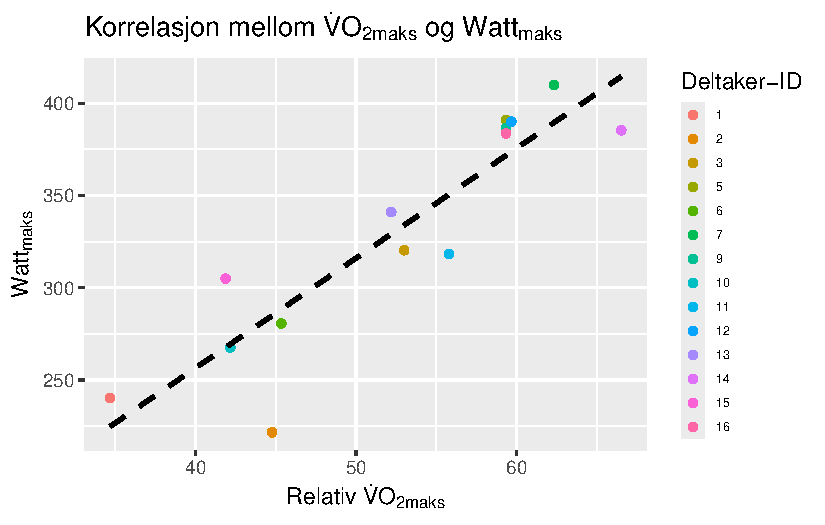
\includegraphics{01-reliability-tools_files/figure-pdf/unnamed-chunk-10-1.pdf}

}

\caption{Figur 1: Hvert punkt = én observasjon}

\end{figure}%

\section{Diskusjon}\label{diskusjon}

På bakgrunn av resultatene vi har observert under testing av
\(\dot{V}O_{2maks}\), kan man slå fast at reliabiliteten til metoden vi
har brukt er ganske god. Resultatene tyder på at vi får målt det vi er
ute etter på en god måte, og det vil variere lite i måle-utstyret fra
gang til gang.

Dette sikrer at vi med ganske god sikkerhet, kan fastslå om et
treningsprogram fungerer, ved å gjøre repeterte tester, med
treningsperioder i mellom.

\bookmarksetup{startatroot}

\chapter{Assignment 2: Regression models, predicting from
data}\label{assignment2}

\section{Introduksjon}\label{introduksjon-2}

En regresjonsmodell er en modell som kvantifiserer forholdet mellom en
eller flere uavhengige variabler og en avhengig variabel. Innen medisin
er regresjon den analysemtoden som er hyppigst anvendt. Det finnes
forskjellige regresjonsmodeller. De vanligste er lineær regresjon,
polynominal regresjon og logistisk regresjon. Hva man har av datasett
vil bestemme hvilken regresjonsmodell som egner seg best å benytte
(Pisică et al. 2022).

En lineær regresjonsmodell er en modell der en kan estimere verdien av
en avhengig variabel basert på verdien av andre kjente uavhengige
variabler (Pisică et al. 2022). I en slik modell benyttes en rett linje
for å lage en modell som beskriver dataen. Følgende funksjon benyttes
for å skape det lineære plottet:

y\textsubscript{i} = b\textsubscript{0} +
b\textsubscript{1}x\textsubscript{i} + e\textsubscript{i}

der y\textsubscript{i} er den avhengige variabelen som kan estimeres ved
å benytte de uavhengige variablene b\textsubscript{1}x\textsubscript{i}
og b\textsubscript{0}. b\textsubscript{0} er skjæringspunktet til grafen
og b\textsubscript{1} er stigningstallet til grafen.

\section{Part 1 - Lactate thresholds}\label{part-1---lactate-thresholds}

\subsection{Metode}\label{metode-1}

Dataene ble organisert i et mer hensiktsmessig format (tidy data) for å
forenkle videre analyse og modellering. Deretter ble ulike
regresjonsmodeller anvendt for å representere dataene. Nye
skjæringspunkter ble tegnet opp for å illustrere treningsintensitet ved
forskjellige laktatnivåer.

\subsection{Resultat}\label{resultat-1}

\begin{figure}

\centering{

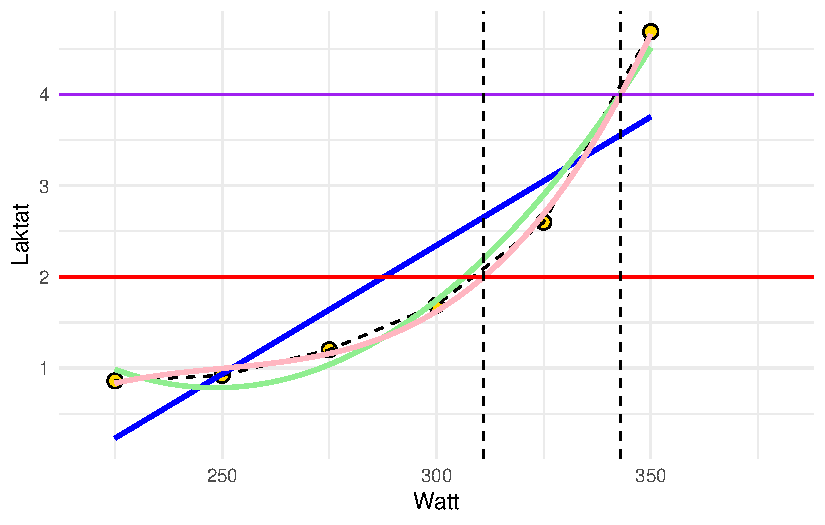
\includegraphics{02-regression-models_files/figure-pdf/fig-fig1-1.pdf}

}

\caption{\label{fig-fig1}Figur 1: Gule punkter = laktat og watt, blå
linje = lineær regresjon, grønn linje = andregradsligning, rosa =
tredjegradsligning.}

\end{figure}%

\subsection{Diskusjon}\label{diskusjon-1}

Vi har valgt å se på subject 10 fra datasettet Cyclingstudy. Vi gjør om
datasettet til tidydata. Dette gjør vi for å gi watt og laktat hver sine
verdier. Vi plotter inn laktatverdier og wattverdier (gule punkter).
Deretter tegner vi en stiplet linje som følger punktene. Vi gjør en
regresjonsanalyse, først en lineær modell (blå linje), deretter en
andregradsligning (grønn) og til slutt en tredjegradsligning (rosa).
Disse bruker vi for å observere hvilken modell som passer best i dette
tilfellet.

For å understreke hvor unøyaktig den lineære modellen er i dette
tilfellet, kan man på øyemål se at laktaten på 300W viser omtrent 2.4
mmol \textbf{×} L-1. Den faktiske laktaten på 300W er 1.69 mmol
\textbf{×} L-1 Figure~\ref{fig-fig1}.

\section{Part 2 - Predicting sizes of DNA
fragments}\label{part-2---predicting-sizes-of-dna-fragments}

\subsection{Metode}\label{metode-2}

For å predikere kalibreringskurven til qPCR, må en rekke prosesser på
molekylærlaboratoriet gjennomføres før dataene kan analyseres i R
Studio.

For å utføre en PCR på en 2\% agarosegel, ble det først tatt helblod fra
en forsøksperson for å ekstrahere DNA. Helblodet gjennomgikk ulike
prosesser hvor forskjellige løsninger og primere ble tilsatt. Dette
resulterte i et PCR-produkt. En elektroforese ble deretter kjørt for å
separere DNA-fragmentene fra PCR-reaksjonen. Etter fullført
elektroforese ble det tatt et bilde av 2\% agarosegelen.

Bildet fra elektroforesen ble analysert ved hjelp av ImageJ/Fiji, og
videre dataanalyser ble utført i R og R Studio. PCR-reaksjoners
effektivitet bestemmes av primerdesign og deres spesifisitet.

\subsection{Resultat}\label{resultat-2}

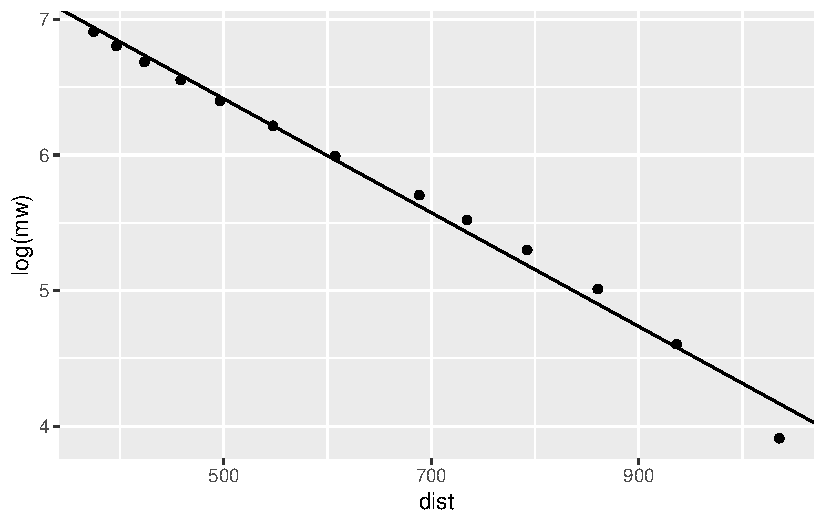
\includegraphics{02-regression-models_files/figure-pdf/unnamed-chunk-3-1.pdf}

\begingroup\fontsize{10}{12}\selectfont

\begin{longtable}[t]{>{}c>{}c>{}c}
\caption{Predikerte molekylvekter for ukjente distanser}\\
\toprule
\cellcolor[HTML]{404080}{\textcolor{white}{\textbf{Båndnummer}}} & \cellcolor[HTML]{404080}{\textcolor{white}{\textbf{Distanse (px)}}} & \cellcolor[HTML]{404080}{\textcolor{white}{\textbf{Predikert molekylvekt (bp)}}}\\
\midrule
\textbf{\cellcolor{gray!10}{1}} & \cellcolor[HTML]{F0F0FF}{\cellcolor{gray!10}{1208.5}} & \cellcolor[HTML]{F0F0FF}{\cellcolor{gray!10}{\cellcolor{red!25}31.22}}\\
\textbf{2} & \cellcolor[HTML]{F0F0FF}{600.5} & \cellcolor[HTML]{F0F0FF}{\cellcolor{yellow!25}400.05}\\
\textbf{\cellcolor{gray!10}{3}} & \cellcolor[HTML]{F0F0FF}{\cellcolor{gray!10}{18.5}} & \cellcolor[HTML]{F0F0FF}{\cellcolor{gray!10}{\cellcolor{green!25}4595.75}}\\
\textbf{4} & \cellcolor[HTML]{F0F0FF}{383.5} & \cellcolor[HTML]{F0F0FF}{\cellcolor{green!25}994.09}\\
\textbf{\cellcolor{gray!10}{5}} & \cellcolor[HTML]{F0F0FF}{\cellcolor{gray!10}{408.5}} & \cellcolor[HTML]{F0F0FF}{\cellcolor{gray!10}{\cellcolor{green!25}895.12}}\\
\addlinespace
\textbf{6} & \cellcolor[HTML]{F0F0FF}{436.5} & \cellcolor[HTML]{F0F0FF}{\cellcolor{green!25}795.93}\\
\textbf{\cellcolor{gray!10}{7}} & \cellcolor[HTML]{F0F0FF}{\cellcolor{gray!10}{470.5}} & \cellcolor[HTML]{F0F0FF}{\cellcolor{gray!10}{\cellcolor{green!25}690.14}}\\
\textbf{8} & \cellcolor[HTML]{F0F0FF}{508.5} & \cellcolor[HTML]{F0F0FF}{\cellcolor{green!25}588.45}\\
\textbf{\cellcolor{gray!10}{9}} & \cellcolor[HTML]{F0F0FF}{\cellcolor{gray!10}{559.5}} & \cellcolor[HTML]{F0F0FF}{\cellcolor{gray!10}{\cellcolor{yellow!25}475.12}}\\
\textbf{10} & \cellcolor[HTML]{F0F0FF}{618.5} & \cellcolor[HTML]{F0F0FF}{\cellcolor{yellow!25}370.95}\\
\addlinespace
\textbf{\cellcolor{gray!10}{11}} & \cellcolor[HTML]{F0F0FF}{\cellcolor{gray!10}{696.5}} & \cellcolor[HTML]{F0F0FF}{\cellcolor{gray!10}{\cellcolor{yellow!25}267.44}}\\
\textbf{12} & \cellcolor[HTML]{F0F0FF}{742.5} & \cellcolor[HTML]{F0F0FF}{\cellcolor{yellow!25}220.51}\\
\textbf{\cellcolor{gray!10}{13}} & \cellcolor[HTML]{F0F0FF}{\cellcolor{gray!10}{798.5}} & \cellcolor[HTML]{F0F0FF}{\cellcolor{gray!10}{\cellcolor{yellow!25}174.34}}\\
\textbf{14} & \cellcolor[HTML]{F0F0FF}{862.5} & \cellcolor[HTML]{F0F0FF}{\cellcolor{yellow!25}133.3}\\
\textbf{\cellcolor{gray!10}{15}} & \cellcolor[HTML]{F0F0FF}{\cellcolor{gray!10}{935.5}} & \cellcolor[HTML]{F0F0FF}{\cellcolor{gray!10}{\cellcolor{red!25}98.14}}\\
\addlinespace
\textbf{16} & \cellcolor[HTML]{F0F0FF}{993.5} & \cellcolor[HTML]{F0F0FF}{\cellcolor{red!25}76.94}\\
\bottomrule
\end{longtable}
\endgroup{}

\subsection{Diskusjon}\label{diskusjon-2}

\section{Part 3 - Interpreting a regression
table}\label{part-3---interpreting-a-regression-table}

\subsection{Metode}\label{metode-3}

\subsection{Resultat}\label{resultat-3}

\begin{figure}[H]

{\centering 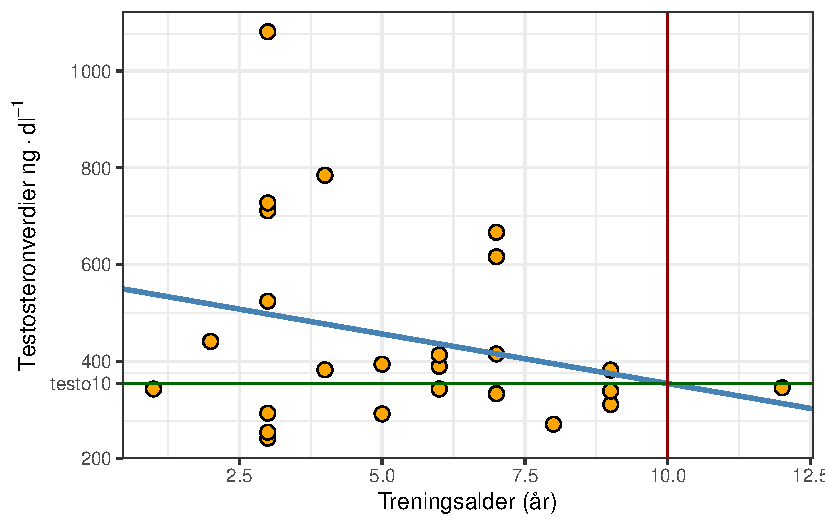
\includegraphics{02-regression-models_files/figure-pdf/tolkning av regresjonsmodell-1.pdf}

}

\caption{Figur 3: Sammenheng mellom treningsalder og testosteronverdier
i blodet}

\end{figure}%

\subsection{Diskusjon}\label{diskusjon-3}

Fra datasettet hypertrophy valgte vi å se på sammenhengen mellom
testosteronkonsentrasjon i blodet (ng \textbf{×} dl-1) og treningsalder
(antall år med trening). Den lineære modellen forteller at
testosteronkonsentrasjonen i blodet synker med 20.51 ng \textbf{×} dl-1
for hvert treningsår. Etter 10 år med trening, estimerer den lineære
modellen et testosteronnivå på 354.26 ng \textbf{×} dl-1.

Analysen av dataene viser en p-verdi på 0,1779, noe som indikerer at det
ikke er statistisk signifikant bevis for en sammenheng mellom
treningsalder og nivået av testosteron i blodet. Siden p-verdien er
høyere enn det vanlige signifikansnivået på 0,05, kan vi ikke avvise
nullhypotesen, som antyder at det ikke er noen betydelig effekt eller
sammenheng mellom de to variablene i dette datasettet. Dette betyr at
variasjonen i testosteronnivåer ikke ser ut til å være relatert til hvor
lenge individene har trent.

I analysen av sammenhengen mellom treningsalder og testosteronnivåer i
blodet ses det en t-verdi på 6.250. Den høye t-verdien på 6.250, og en
p-verdi på 0,1779. Denne p-verdien er høyere enn det vanlige
signifikansnivået på 0,05, noe som betyr at vi ikke har tilstrekkelig
statistisk bevis for å avvise nullhypotesen. Selv om t-verdien indikerer
en mulig sammenheng mellom treningsalder og testosteronnivå, er det ikke
nok evidens til å konkludere med at denne sammenhengen er signifikant.
Dermed kan vi konkludere med at selv om det kan være en tendens til en
sammenheng mellom treningsalder og testosteronnivåer, er resultatene fra
denne analysen ikke sterke nok til å si at treningsalder har en reell
effekt på testosteronnivåene i blodet.

\bookmarksetup{startatroot}

\chapter{Assignment 3: Drawing inference from statistical models, and
statistical power}\label{assignment3}

This assignment is set up as a statistical laboratory, we will perform
simulations and your assignment is to interpret and explain the results.
Create a report based on the code used in the lab and make sure you
answer the specified questions (1-8). You can be as creative as you want
and explore the results further.

\section{Spørsmål:}\label{spuxf8rsmuxe5l}

\subsection{Estimate}\label{estimate}

Estimate er et tall vi får, basert på utregning via en lineær modell.
Tallet vi får representerer en gjetning av gjennomsnittet til variabelen
``y'' i vårt utvalg. \textbf{SE} er standardfeil, som sier noe om hvor
stor usikkerhet det er tilknyttet estimatet vårt. Usikkerheten vi
snakker om her forteller noe om hvor mye dette gjennomsnittet potensielt
kan avvike fra populasjonsgjennomsnittet. \textbf{T-verdien} sier her
noe om forholdet mellom estimatet vårt (\textbf{estimate}) og
standardfeilen (\textbf{SE}). \textbf{P-verdi} sier noe om hvor stor
sannsynlighet det er for at vi observerer et resultat som er like
ekstremt, eller enda mer ekstremt enn hva vi har fått i dette tilfellet.
I vårt tilfelle har vi en høy \textbf{P-verdi} noe som forteller at vi
ikke kan forkaste nullhypotesen, da det ikke er noen forskjell i fra
null.

\subsection{m1 vs m2}\label{m1-vs-m2}

Forskjellen mellom studiene kommer fra størrelsen på utvalget som er
brukt i de to forskjellige. I \emph{m1} er det brukt ett mye mindre
utvalg, noe som fører til større usikkerhet rundt resultatene. I
\emph{m2} er det brukt et større utvalg, som gjør at det estimerte
gjennomsnittet blir nærmere populasjonsgjennomsnittet og standardfeilen
blir dermed mindre. Dette gir i vårt tilfelle en høyere \textbf{t-verdi}
og en lavere \textbf{p-verdi}.

\subsection{Shaded areas}\label{shaded-areas}

Vi bruker de grå feltene for å vise de ekstreme verdiene vi har fra
testen vår. Jo lenger ut i halene vi kommer, desto større sannsynlighet
er det for at dette er et uvanlig resultat å se.

\subsection{\texorpdfstring{Standard deviation of \textbf{estimate} and
avg. \textbf{se} for each
study.}{Standard deviation of estimate and avg. se for each study.}}\label{standard-deviation-of-estimate-and-avg.-se-for-each-study.}

Standard deviation for modellen med 8 i population er 1.07, mens det for
modellen med 40 i population er 0.48. Når det kommer til gjennomsnittlig
standardfeil ligger den på 1.02 for modellen med 8 i population, mens
den for modellen med 40 i population ligger på 0.47. Grunnen til at
tallene er såpass like som de er for \textbf{SD} og \textbf{avg se} er
at begge beregningene er mål på variasjon. I denne sammenhengen er
standardfeilen et mål på hvor mye gjennomsnittet avviker fra det sanne
populasjonsgjennomsnittet.

\subsection{P-value histogram}\label{p-value-histogram}

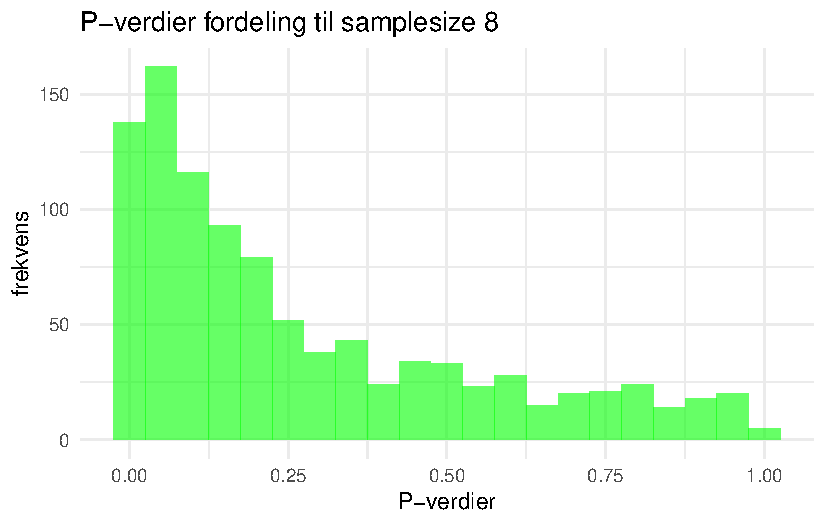
\includegraphics{03-statistical-inference_files/figure-pdf/P-verdi histogram SS8-1.pdf}

Når vi ser histogrammet for modellen med utvalgsstørrelse på 8, ser vi
tydelig at det er mange observasjoner av høye p-verdier. Dette
gjenspeiler den lave statistiske poweren vi får av å gjøre studier med
en så liten utvalgsstørrelse.

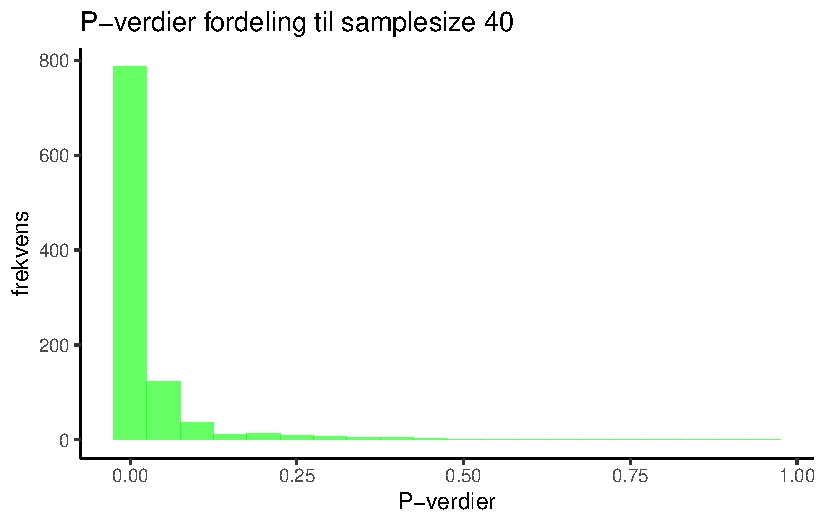
\includegraphics{03-statistical-inference_files/figure-pdf/P-verdi histogram SS40-1.pdf}

På histogrammet med utvalgsstørrelse på 40 ser vi at det er en mye
større samling av observasjoner på lave p-verdier. Dette gjenspeiler det
vi vet om at en større utvalgsstørrelse gir en større statistisk power.

\subsection{Antall studier med statistisk
signifikans}\label{antall-studier-med-statistisk-signifikans}

I studiene med utvalgsstørrelse på 8 ser vi at det er 227 studier som
viser statistisk signifikans, mens det i studiene med utvalgsstørrelse
på 40 er hele 865 studier som viser statistisk signifikans. Dette gir et
godt bilde på hvor mye utvalgsstørrelsen har å si for resultatet i
utregningen vår. I mitt tilfelle har jeg valgt å sette terskelen for
signifikans (p-verdi) til 0.05.

\subsection{Power of a one-sample
t-test}\label{power-of-a-one-sample-t-test}

Når vi gjennomfører utregningen ser vi at studiene med lav
utvalgsstørrelse (8) får en mye lavere statistisk styrke (0.232) enn
studiene med utvalgsstørrelse på 40 (0.869). Svarene vi får av disse
utregningene støtter det vi tidligere har funnet ut, at dersom vi har et
større utvalg, er det større sannsynlighet for at vi ser en faktisk
effekt, og at det ikke er en tilfeldighet at vi har funnet det vi har i
studien. I dette tilfelle vil vi da få en 86.9\% sjanse for å oppdage en
sann effekt.

\subsection{Med signifikansnivå på 0.05 hvor mange studier gir ``falsk
positiv'' ved gjennomføring av mange repeterte
studier?}\label{med-signifikansnivuxe5-puxe5-0.05-hvor-mange-studier-gir-falsk-positiv-ved-gjennomfuxf8ring-av-mange-repeterte-studier}

Ved å gjøre 1000 repeterte studier, vil vi få omtrent 50 falske positive
hvis vi setter signifikansnivået til 0.05. I min utregning fikk jeg da
49 for studiene med utvalgsstørrelse på 8 og 59 på studiene med
utvalgsstørrelse 40. Om jeg endrer signifikansnivået og setter alpha
enda lavere vil resultatet endre seg litt. Med en signifikansverdi på
0.025 vil det i studiene med utvalgsstørrelse 8 gi meg 30 falske
positive, mens det på studiene med 40 i utvalgsstørrelse gir 22 falske
positive.

\bookmarksetup{startatroot}

\chapter{Assignment 4: Study designs}\label{assignment-4-study-designs}

\section{Introduksjon}\label{introduksjon-3}

Formålet med denne sammenligningen er å se på ulikheter rundt de
metodiske valgene ved de ulike studiene. Felles for studiene jeg har
valgt å se på er at de alle ser på effekten av bolklagt
utholdenhetstrening sett mot tradisjonell utholdenhetstrening og
effekten av dette på VO\textsubscript{2maks}. Videre blir det sett på
styrker og svakheter ved studiedesign, statistiske analyser og
resultater. Det vil til slutt bli gitt noen anbefalninger til fremtidige
studier.

\section{Metode}\label{metode-4}

Det ble valgt ut fem ulike studier, som alle ser på effekten av
blokkperiodisering av utholdenhetstrening på VO\textsubscript{2maks}.
Studienes styrker og svakheter ble analysert, og det ble spesielt
vektlagt studiedesign og statistiske analyser. Studiedesignenes evne til
å måle relevante utfall ble vurdert, samt i hvor stor grad det ble tatt
høyde for eksterne variabler som kunne påvirke resultatene.

\section{Resultat}\label{resultat-4}

Den første studien det ble sett på (Rønnestad, Hansen, and Ellefsen
2014) brukte et kontrollert design med objektive målinger som
VO\textsubscript{2maks}, anvendbarheten er kanskje ikke så god da
utvalgsstørrelsen er såpass liten som den er og det er manglende
kontroll for eksterne faktorer.

Den andre studien (Rønnestad et al. 2014) hadde et robust eksperimentelt
design med godt definerte kontrollgrupper og brukte gjentatte målinger
for å spore prestasjonsendringer. Likevel var ekstern validitet en
utfordring på grunn av spesifisiteten til utvalget, og tidsrammen for
kort til å vurdere langsiktige effekter.

Studie nummer tre (Breil et al. 2010) implementerte blokkperiodisering
og benyttet et bredt spekter av ulike prestasjonsmål. Den korte
intervensjonsperioden og det lave antallet kvinnelige deltakere utgjorde
imidlertid svakheter som kan ha påvirket representativiteten og
konklusjonene.

Den fjerde studien (Rønnestad et al. 2016) benyttet avanserte
statistiske analyser og hadde et langsiktig design, men en begrenset
utvalgsstørrelse og fokus på eliteutøvere reduserte generaliserbarheten
av funnene i studien.

Studie fem (Solli, Tønnessen, and Sandbakk 2019) brukte et omfattende
design med både fysiologiske og prestasjonsbaserte utfall. Svakheten var
spesifisiteten til deltakerutvalget, og det var behov for en bedre
sammenheng mellom de statistiske testene og forskningsspørsmålene i
studien.

\section{Diskusjon}\label{diskusjon-4}

Studiene generelt sett har god intern validitet, grunnet robuste
studiedesign og gode kontrollgrupper. Den eksterne validiteten derimot
er det verre med, dette med bakgrunn i at det er små utvalgsstørrelser
og spesifikke grupper, eksempelvis eliteutøvere som er testet. Dette
reduserer generaliserbarheten til studiene. Studiene har også benyttet
seg av noe ulik varighet på treningsintervensjonene som har blitt brukt
i studiene. Dette gjør at det blir vanskeligere å trekke konlusjoner
rundt langsiktige effekter av treningen. Generelt sett er det valgt gode
statistiske analyser i studiene. Det kunne dog vært gjort mer detaljert
begrunnelse for valg av statistiske tester i enkelte av studiene.

\section{Konklusjon}\label{konklusjon}

Det bør i fremtidige studier fokuseres på å øke størrelsesutvalget, og
inkludere mer varierte populasjoner for å forbedre generaliserbarheten
og gjøre funnene mer anvendbare for hele befolkningen. Det kan med
fordel også brukes lengre oppfølgingstider for å vurdere langsiktige
effekter av treningsintervensjoner. Valg av statistiske analyser bør
være tett koblet til forskningsspørsmålene for å sikre at de gir
meningsfulle og presise svar.

\bookmarksetup{startatroot}

\chapter{Assignment 5: Analyzing repeated measures
experiments}\label{assignment-5-analyzing-repeated-measures-experiments}

\section{Introduksjon}\label{introduksjon-4}

Et styrketreningsprogram kan bestå av mange ulike variabler, som i
teorien skal påvirke adaptasjoner. Volum, intensitet, frekvens,
pauselengder, samt ernærning, kontraksjonstype og kontraksjonshastighet
er eksempler på dette. At vi har så mange forskjellige variabler, gjør
at vi har muligheten til å gjøre endringer på uttallige forskjellige
måter for å manipulere og tilpasse treningsprogrammer. Volum i
styrketrening er et mye debattert tema, her er det spesielt ett sett,
mot flere sett som har fått mye oppmerksomhet (Carpinelli and Otto
1998).

Flere studier har vist at økt treningsvolum er fordelaktig for både
muskelstyrke og muskelvekst (hypertrofi) (Sooneste et al. 2013; Radaelli
et al. 2015). Likevel finnes det forskning som indikerer at lavt volum
kan gi styrke- og masseøkninger som er sammenlignbare med de som oppnås
ved moderat volum (Cannon and Marino 2010; Mitchell et al. 2012). Denne
variasjonen i studieresultater skyldes sannsynligvis en kombinasjon av
små utvalgsstørrelser og individuelle forskjeller. Studiedesign som
sammenligner ulike treningsvolumer hos samme person kan teoretisk sett
bidra til å håndtere disse begrensningene. I flere studier som
undersøker ett sett kontra tre sett, er det også forskjeller i
intensitet og hvilke øvelser som benyttes (Marx et al. 2001; Messier and
Dill 1985).

Formålet med analysene i denne rapporten var å sammenligne effekten av
ett sett versus flere sett på både muskelstyrke og hypertrofi. Med tanke
på de metodiske utfordringene i studier som sammenligner ett sett med
flere sett, er følgende hypotese formulert: Tre sett vil være mer
effektive for å forbedre maksimal muskelstyrke og øke muskelmasse
sammenlignet med ett sett.

\section{Metode}\label{metode-5}

\subsection{Forsøkspersoner og
studiedesign}\label{forsuxf8kspersoner-og-studiedesign}

Det ble rekruttert 41 mannlige og kvinnelige deltakere, kriteriene for å
bli inkludert i studien var å ikke røyke, samt være mellom 18 og 40 år.
Eksklusjonskriteriene var at vedkommende hadde trent mer enn én
styrkeøkt i uken, i løpet av de siste 12 månedene før intervensjonen
startet, intoleranse mot bedøvelse, reduksjon i muskelstyrke grunnet
skade og bruk av reseptbelagte medisiner som i verstefall kunne påvirke
treningsadaptasjoner. Det var syv deltakere som ble ekskludert fra
analysene som ble gjort, fordi de ikke fullførte minst 85\% av den
planlagte treningen. Samtlige inkluderte deltakere rapporterte at de
hadde erfaring med idrettsaktiviteter fra tidligere. Blant deltakerne
var det tjue av dem som drev med fysisk trening da de meldte seg på
studien; blant disse var det ti av dem som drev sporadisk styrketrening,
men felles for dem var at ingen trente mer enn én gang i uken.

Intervensjonen besto av 12 uker med styrketrening for hele kroppen,
denne ble fullført av samtlige deltakere fra september til november. Det
ble gjort en randomisering på hvert ben hos deltakerne, for å muliggjøre
differensiering av treningsvolum hos samme deltaker. Hver deltaker fikk
da tilfeldig tildelt enten ett eller tre sett, til hvert av beina sine,
så hver person fikk fulgt begge protokollene. Det ble gjort måling av
muskelstyrke ved baseline, underveis (uke 3, 5 og 9) og etter
intervensjonen. Målinger av kroppssammensetning ble utført før og etter
intervensjonen.

\subsection{Treningsprotokoll}\label{treningsprotokoll}

Styrkeøvelsene ble gjennomført i denne rekkefølgen: unilateral
beinpress, beincurl og kneekstensjon. Ett sett op det ene beinet, og tre
sett på det andre beinet, ut i fra randomiseringen. Beinet som skulle
trene ett sett, ble trent mellom andre og tredje sett på beinet som
trente tre sett. Når øvelsene på beina var gjennomført, trente de også
to sett av bilateral benkpress, nedtrekk og enten sittende roing eller
skulderpress (skulderpress og sittende roing varierte fra økt til økt
(annenhver gang)). Pauselengde mellom settene var mellom 1.5 og 3
minutter. Det ble gjort en gradvis økning i treningsmotstanden utover
treningsintervensjonen. Deltakerne startet med 10 RM de to første ukene,
deretter 8 RM i tre uker og 7 RM i syv uker. Etter økt nummer ni, ble
motstanden redusert på én av de tre øktene som var ukentlig. Dette var
en reduksjon tilsvarende 90 \% (av motstanden) fra forrige økt på den
gitte øvelsen. Deltakeren hadde fortsatt mål om samme repetisjonsantall.
Det ble satt et minimum om 48 timer fra fullført økt med maksimal innsat
og frem til neste økt. Etter styrkeøktene med redusert motstand var det
minst 24 timer til den neste økten. For å sørge for best mulig
umiddelbar resitusjon fikk deltakerne en standardisert drikke etter hver
gjennomførte økt med 0.15 g/kg protein, 1.2 g/kg karbohydrater og 0.5
g/kg fett.

\subsection{Målinger av muskelstyrke og
hypertrofi}\label{muxe5linger-av-muskelstyrke-og-hypertrofi}

Maksimal styrke er definert som den motstanden man maksimalt klarer å
løfte en repetisjon av (1 RM) i beinpress og kneekstensjon. Det ble
gjort en spesifikk oppvarming med ti, seks og tre repetisjoner på
henholdsvis 50, 75 og 85 \% av forventet 1 RM. Motstanden ble deretter
økt progressivt helt til deltakeren ikke lenger klarte å løfte mer. Den
høyeste motstanden med godkjent repetisjon er definert som 1 RM.
Deltakerne fikk fire til seks forsøk hver.

Testene ble gjennomført to ganger ved baseline, med fire dager mellom.
Den høyeste enkeltverdien de oppnådde på disse to dagene er brukt i
analysene. Styrketestene ble gjort minst 48 timer etter siste
gjennomførte økt etter intervensjonen. Ikke alle deltakerne (n = 18)
gjorde styrketestene underveis i intervensjonen (uke to, fem og ni). Det
ble prioritert trening for de andre deltakerne, dersom de gikk glipp av
enten test eller trening grunnet sykdom eller andre utfordringer.
Testene underveis er derfor ikke inkludert i analysene for at det skulle
være et større utvalg i analysene. Derfor er resultatene før og etter
treningsintervensjonen det som er tatt med i analysene.

\bookmarksetup{startatroot}

\chapter{Endre under her}\label{endre-under-her}

Kroppssammensetning for bestemmelse av mager muskelmasse er bestemt ved
dual-energy X-ray absorptiometry (DXA) før og etter intervensjonen
(Lunar Prodigy, GE Healthcare, Oslo, Norway). Før DXA-målinger fikk
deltakerne beskjed om å faste 2 timer og avstå fra krevende fysisk
aktivitet i 48 timer. Det var også minimum 48 timer fra siste styrkeøkt
til DXA-måling.

\subsection{Dataanalyser og
statistikk}\label{dataanalyser-og-statistikk}

Statiske analyser er gjort i R studio (Posit team 2023). Det er gjort
enkle lineære regresjonsmodeller på differansen mellom gruppene (ett
sett \& flere sett) i endring av styrke og muskelmasse i løpet av
intervensjonen. For maksimal styrke er det gjort analyser på øvelsene
beinpress og kneekstensjon. Muskelmasse er målt som endringen i mager
muskelmasse i beinet som har trent ett mot beinet som har trent tre
sett.

\section{Resultater}\label{resultater}

DXA-resultatene viste at gjennomsnittlig differanse mellom ett og tre
sett var 122.79 (95 \% KI: {[}8.59-237{]}, p = 0.04). Også for
styrkeøvelsene var forbedringen i 1RM i gjennomsnitt større for det
beinet som hadde trent flere sett. I beinpress var forskjellen 7.22 (95
\% KI: {[}0.9-13.5{]}, p = 0.026), mens for kneekstensjon var det 3.6
(95 \% KI: {[}1.4-5.8{]}, p = 0.002) differanse.

Tabellen nedenfor viser nivået ved baseline for styrkeøvelsene og mager
muskelmasse.

\begingroup
\fontsize{12.0pt}{14.4pt}\selectfont
\setlength{\LTpost}{0mm}

\begin{longtable}{lrrr}

\caption{\label{tbl-pre}Resultater fra pre-test}

\tabularnewline

\toprule
Volum & Magermasse (g) & Beinpress (kg) & Kneekstensjon (kg) \\ 
\midrule\addlinespace[2.5pt]
multiple & 8,603.5 ± 2,032.9 & 208.1 ± 76.4 & 69.2 ± 23.3 \\ 
single & 8,589.0 ± 2,021.0 & 217.9 ± 76.1 & 74.3 ± 25.5 \\ 
\bottomrule

\end{longtable}

\begin{minipage}{\linewidth}
\emph{Data er presentert som gjennomsnitt ± standardavvik.}\\
\end{minipage}
\endgroup

Figuren viser om det er en sammenheng mellom prosentvis endring i
muskelmasse og 1RM beinpress. 0.5 \% av endringen i 1RM beinpress kan
forklares med endringen i muskelmasse (R = 0.005 \& p = 0.59).

\begin{figure}

\centering{

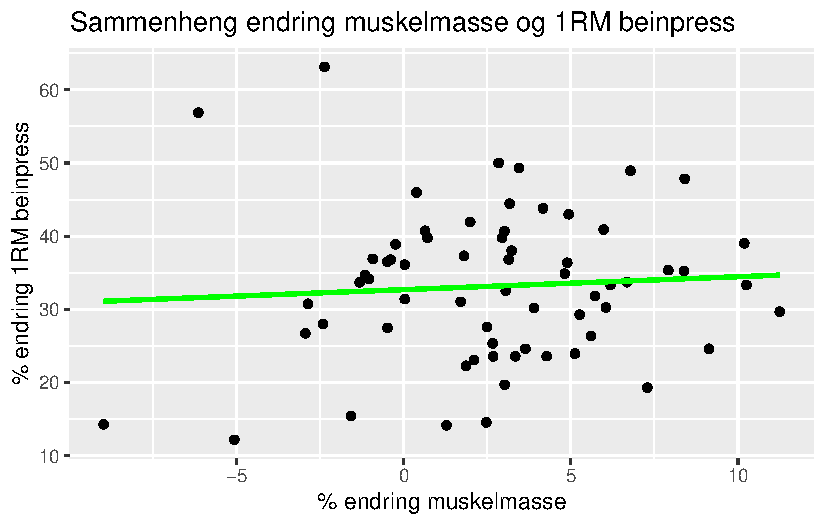
\includegraphics{05-repeated-measurements_files/figure-pdf/fig-figur1-1.pdf}

}

\caption{\label{fig-figur1}Figur som viser en lineær regresjonsmodell
med endring i muskelmasse som prediktor variabel for endring i 1RM
beinpress.}

\end{figure}%

\section{Diskusjon}\label{diskusjon-5}

I det beinet som trente tre sett, så man at det var mer hypertrofi og
større økning i styrke, målt i de to øvelsene, sammenlignet med de som
trente ett sett. Prosentvis endring i magermasse var høyere ved 3 sett,
henholdsvis 3.1 ± 4.4 \% mot ett sett, som økte 1.9 ± 3.5 \%. Man har
sett det samme i en metaanalyse, som så at to til tre sett og fire til
seks sett ga bedre resultat på effektstørrelse enn ett sett (ingen
forskjell mellom to til tre og fire til seks sett) (Krieger 2009). Vi
skal være litt forsiktige med å trekke konlusjoner basert på
metaanalyser, men mange andre studier sammenligner grupper med
forskjellige deltakere og ikke samme deltaker med ulikt treningsvolum på
to forskjellige bein (Starkey et al. 1996). Dette gjør at man ikke får
tatt høyde for biologiske variasjoner hos de ulike individene, dermed
blir det vanskelig å sammenligne ulikt volum. Økningen i muskelmasse kan
i analysene fra denne rapporten ikke forklare økningen i 1 RM beinpress
når begge bein ble inkludert i korrelasjonsanalysen.

Til tross for at det ikke var noen sammenheng, så man også em større
økning i styrke, i beinpress ved tre sett kontra ett sett (den
prosentvise endringen på henholdsvis 34.4 ± 10.5 \& 31.9 ± 10). Man så
det samme på kneekstensjon, tre sett økte her 32.5 ± 9.1 \%, ett sett
derimot økte med 30.4 ± 8.8 \%.

Som konklusjon ut i fra de gjennomførte analysene fra rapporten, kan vi
si at responsen på styrke og hypertrofi følger et dose-volum forhold.
Dette vil si at tre sett er mer gunstig enn ett sett for ikke-røykende,
utrente kvinner og menn mellom 18 og 40 år.

\bookmarksetup{startatroot}

\chapter{Philosophy of science}\label{philosophy-of-science}

\section{Induksjon}\label{induksjon}

Induksjon er en prosess som blir brukt for å trekke konklusjoner basert
på observasjoner vi har gjort (Thurén 2022). Metoden, eller prosessen
blir gjerne brukt for å trekke generelle konklusjoner angående hvordan
verden er satt sammen og hvordan den fungerer. Konklusjonene baserer seg
på spesifikke observasjoner som har blitt gjort tidligere, og
observasjonene har gjerne blitt testet om igjen, og om igjen for å sørge
for at ting ikke har skjedd ved én tilfeldighet.

Det finnes både fullstendig og ufullstendig induksjon. Et eksempel på
fullstendig induksjon er ved valg, valgresultatet baserer seg på
induksjon. Alle stemmesedlene blir telt opp og vi kan konkludere med at
kandidaten som har fått flest stemmer, vinner valget. Ved fullstendig
induksjon kan vi være helt sikre på at konklusjonen vi har kommet frem
til er rett, siden vi har sett på alle stemmesedlene. Ved ufullstendig
induksjon baserer man seg på et begrenset antall observasjoner og
trekker en generell konklusjon deretter. Ved ufullstendig induksjon vil
det alltid være en fare for at konklusjonen er usann, siden man ikke
undersøker alle relevante tilfeller.

Hume mener på sin side at induksjon rett og slett ikke er så mye verdt.
I Humes´ øyne er det ingen logisk forklaring til at fremtiden vil
fortsette å være lik fortiden i all fremtid. Erfaringer vi har gjort oss
tidligere sier heller ikke noe om fremtiden, selv om det gir en god
pekepinn. Selv om to biler krasjer i et bestemt kryss i dag, betyr ikke
det at to biler vil krasje i det samme krysset i morgen. Hume
konkluderer med at induksjon kun er basert på vaner og/eller
forventninger og at det ikke er basert på rasjonell grunn.

En innvendig mot Humes premiss er at vi mennesker klarer å gjøre gode
resonnementer, gjenkjenne mønstre og tenke logisk. Med bakgrunn i dette
kan vi si at våre forventninger om fremtiden ikke kun er baser på
forventninger og vaner, men fra en dypere rasjonell forståelse av
verden. At ting har blitt som de har, er et resultat av den stadige
evolusjonen og utviklingen vi har hatt som menneskehet. Vi og verden har
utviklet oss for å stadig bedre vår overlevelsesevne. Og dermed vil vi
også fortsette å utvikle oss videre.

Hume ville i dette tilfellet antakelig svart med noe som at; selv om vi
i all tid så langt har utviklet oss som menneskehet, og verden stadig
har tatt fremskritt, betyr det ikke at vi vil fortsette med det i
morgen. Selv om all fornuft tyder på at morgendagen vil ligne på dagen i
går, siden dagen før der lignet på dagen i går, betyr det ikke at det
vil være sånn. Selv om vi mennesker har blitt gode på å kjenne igjen
mønstre, kan man fortsatt ikke forutse hvordan morgendagen blir. Det vet
vi kun i morgen.

\section{Falsifikasjonisme}\label{falsifikasjonisme}

Hovedessensen av prinsippet om falsifikasjon, eller falsifikasjonisme
handler om at vi i vitenskapen ikke bør prøve å finne argumenter for at
noe stemmer, men at vi heller bør prøve å falsifisere, altså bevise at
noe er usant. Karl Popper var opptatt av at teorier skulle kunne
motbevises ved hjelp av eksperimenter, eller observasjoner. Et eksempel
vi kan bruke fra idretten er teorien om at bruken av høydetrening kan
forbedre utholdenhetsprestasjonen. Hvis man har to forskjellige grupper,
en på høydetrening og en uten høydetrening. Og det ikke ses noen
forskjell i utholdenhetsprestasjon, kan hypotesen om høydetrening
falsifiseres. Hvis teorier kommer seg gjennom mange forsøk på
falsifikasjon, kan vi se på den som at den foreløpig er korrekt, men
aldri som endelig bekreftet. Popper gikk på sin side så langt, som å si
at søken etter bekreftelser på hypoteser er selve kjennetegnet på
pseudovitenskap.

Et problem med falsifikasjonisme, hentet fra idretten er effekten av
varmetrening på utholdenhetsprestasjon. Det har i dag blitt vanligere og
vanligere å drive med varmetrening, enten i oppvarmet rom eller ved bruk
av varmedrakt (for eksempel ullundertøy under regntøy). Det er mye
diskutert hva slags effekt dette kan ha på utholdenhetsprestasjonen,
også i konkurranser eller tester hvor det er normale forhold (hverken
oppvarmet rom eller varmedrakt i bruk). Det er en del andre variabler
som spiller inn her, spesielt individuelle forskjeller som gjøres blant
utøvere både underveis og i ettertid av en varmetreningsøkt. Eksempler
på dette er hydrering underveis og i etterkant, hvile og jern som
kosttilskudd. Dette gjør det vanskelig å teste denne hypotesen på en
falsifiserbar måte. En mulig løsning på dette problemet er å gjøre lange
kontrollerte studier der utøvere gjennomgår trening i varme forhold
(varmekammer/varmedrakt), med en stor nok kontrollgruppe som ikke gjør
noen form for varmetrening. I tillegg bør man i dette tilfellet sørge
for kontrollert oppfølging av både hydrering (sørge for at deltakerne
drikker lik mengde), hvile og andre faktorer som kan påvirke effekten av
varmetreningen. Dette er ulike tiltak som gjør at hypotesen blir mer
falsifiserbar.

Et annet eksempelproblem innenfor idrettsforskning og falsifikasjonisme
er som følger. Det settes opp et prosjekt som skal se på utvikling av
utholdenhet og styrke hos en rekke deltakere. Det gjøres baselinetester
før en treningsintervensjon på 12 uker. Etter de 12 ukene med trening er
gjennomført gjennomføres det nye tester for å se hvordan deltakerne nå
presterer. Halve gruppen har trent harde intervaller, og den andre
halvdelen har trent rolig trening. Gruppen som har gjennomført
intervalltrening har oppnådd mest fremgang, men problemet er at vi ikke
har tatt høyde for individuelle forskjeller blant deltakerne som er med.
En mulig løsning på dette problemet er at vi lar deltakerne få en 12
ukers washout-periode hvor det ikke blir gjennomført noe trening. Man
gjør nye baselinetester for å se om deltakerne nå har mistet
treningsadaptasjonene de opparbeidet seg i forkant. Vi gjennomfører nå
12 nye uker med trening, og deltakerne har nå byttet om, de som trente
intervalltrening under forrige intervensjon får nå rolig trening denne
gangen. På denne måten tar vi høyde for individuelle forskjeller,
ettersom vi nå har byttet om på deltakerne. Dette er en måte å gjøre
hypotesen mer falsifiserbar på.

Et tredje forsøk fra idrettsverden er placeboeffekt, det finnes mye
forskning gjort på kosttilskudd innenfor idretten. Hvis en utøver tror
man får et kosttilskudd som skal gi en forventet bedring i prestasjon
kan dette være nok til at man presterer bedre. Dette gjør det vanskelig
å falsifisere hypoteser. En mulig løsning på dette problemet er å gjøre
double blinded eller dobbeltblinda eksperimenter, så hverken forsker
eller forsøksperson vet om man får placebo eller om man får det faktiske
kosttilskuddet. Dette gjør hypotesen mer falsifiserbar, for hvis man i
dette tilfellet også finner effekt, kan man med ganske god sannsynlighet
si at det er på grunn av kosttilskuddets virkemiddel og ikke at utøveren
tror man har fått tilskuddet.

\bookmarksetup{startatroot}

\chapter{Molecular Laboratory report}\label{molecular-laboratory-report}

Select one laboratory assignment and write a detailed report.

\bookmarksetup{startatroot}

\chapter*{References}\label{references}
\addcontentsline{toc}{chapter}{References}

\markboth{References}{References}

\phantomsection\label{refs}
\begin{CSLReferences}{1}{0}
\bibitem[\citeproctext]{ref-Bassett}
Bassett, D R, Jr, and E T Howley. 2000. {``Limiting Factors for Maximum
Oxygen Uptake and Determinants of Endurance Performance.''} \emph{Med.
Sci. Sports Exerc.} 32 (1): 70--84.

\bibitem[\citeproctext]{ref-Breil2010-mr}
Breil, Fabio A, Simone N Weber, Stefan Koller, Hans Hoppeler, and
Michael Vogt. 2010. {``Block Training Periodization in Alpine Skiing:
Effects of 11-Day {HIT} on {VO2max} and Performance.''} \emph{Eur. J.
Appl. Physiol.} 109 (6): 1077--86.

\bibitem[\citeproctext]{ref-cannon2010}
Cannon, Jack, and Frank E. Marino. 2010. {``Early-Phase Neuromuscular
Adaptations to High- and Low-Volume Resistance Training in Untrained
Young and Older Women.''} \emph{Journal of Sports Sciences} 28 (14):
1505--14. \url{https://doi.org/10.1080/02640414.2010.517544}.

\bibitem[\citeproctext]{ref-carpinelli1998}
Carpinelli, Ralph N., and Robert M. Otto. 1998. {``Strength Training:
Single Versus Multiple Sets.''} \emph{Sports Medicine} 26 (2): 73--84.
\url{https://doi.org/10.2165/00007256-199826020-00002}.

\bibitem[\citeproctext]{ref-Halperin}
Halperin, Israel, David B Pyne, and David T Martin. 2015. {``Threats to
Internal Validity in Exercise Science: A Review of Overlooked
Confounding Variables.''} \emph{Int. J. Sports Physiol. Perform.} 10
(7): 823--29.

\bibitem[\citeproctext]{ref-RN130}
Hopkins, W. G. 2000. {``Measures of Reliability in Sports Medicine and
Science.''} Journal Article. \emph{Sports Med} 30 (1): 1--15.
\url{http://www.ncbi.nlm.nih.gov/pubmed/10907753}.

\bibitem[\citeproctext]{ref-Joyner}
Joyner, Michael J, and Edward F Coyle. 2008. {``Endurance Exercise
Performance: The Physiology of Champions.''} \emph{J. Physiol.} 586 (1):
35--44.

\bibitem[\citeproctext]{ref-krieger2009}
Krieger, James W. 2009. {``Single Versus Multiple Sets of Resistance
Exercise: A Meta-Regression.''} \emph{Journal of Strength and
Conditioning Research} 23 (6): 1890--1901.
\url{https://doi.org/10.1519/JSC.0b013e3181b370be}.

\bibitem[\citeproctext]{ref-marx2001}
Marx, James O., Nicholas A. Ratamess, Bradley C. Nindl, Lincoln A.
Gotshalk, Jeff S. Volek, Keiichiro Dohi, Jill A. Bush, et al. 2001.
{``Low-Volume Circuit Versus High-Volume Periodized Resistance Training
in Women:''} \emph{Medicine and Science in Sports and Exercise}, April,
635--43. \url{https://doi.org/10.1097/00005768-200104000-00019}.

\bibitem[\citeproctext]{ref-messier1985}
Messier, Stephen P., and Mary Elizabeth Dill. 1985. {``Alterations in
Strength and Maximal Oxygen Uptake Consequent to Nautilus Circuit Weight
Training.''} \emph{Research Quarterly for Exercise and Sport} 56 (4):
345--51. \url{https://doi.org/10.1080/02701367.1985.10605339}.

\bibitem[\citeproctext]{ref-mitchell2012}
Mitchell, Cameron J., Tyler A. Churchward-Venne, Daniel W. D. West,
Nicholas A. Burd, Leigh Breen, Steven K. Baker, and Stuart M. Phillips.
2012. {``Resistance Exercise Load Does Not Determine Training-Mediated
Hypertrophic Gains in Young Men.''} \emph{Journal of Applied Physiology}
113 (1): 71--77. \url{https://doi.org/10.1152/japplphysiol.00307.2012}.

\bibitem[\citeproctext]{ref-Pisica2022}
Pisică, Dana, Ruben Dammers, Eric Boersma, and Victor Volovici. 2022.
{``Tenets of Good Practice in Regression Analysis. A Brief Tutorial.''}
\emph{World Neurosurg.} 161 (May): 230--239.e6.

\bibitem[\citeproctext]{ref-rstudio}
Posit team. 2023. \emph{RStudio: Integrated Development Environment for
r}. Boston, MA: Posit Software, PBC. \url{http://www.posit.co/}.

\bibitem[\citeproctext]{ref-radaelli2015}
Radaelli, Regis, Steven J. Fleck, Thalita Leite, Richard D. Leite, Ronei
S. Pinto, Liliam Fernandes, and Roberto Simão. 2015. {``Dose-Response of
1, 3, and 5 Sets of Resistance Exercise on Strength, Local Muscular
Endurance, and Hypertrophy.''} \emph{Journal of Strength and
Conditioning Research} 29 (5): 1349--58.
\url{https://doi.org/10.1519/JSC.0000000000000758}.

\bibitem[\citeproctext]{ref-Ronnestad2014-xg}
Rønnestad, B R, S Ellefsen, H Nygaard, E E Zacharoff, O Vikmoen, J
Hansen, and J Hallén. 2014. {``Effects of 12 Weeks of Block
Periodization on Performance and Performance Indices in Well-Trained
Cyclists.''} \emph{Scand. J. Med. Sci. Sports} 24 (2): 327--35.

\bibitem[\citeproctext]{ref-Ronnestad2014-bu}
Rønnestad, B R, J Hansen, and S Ellefsen. 2014. {``Block Periodization
of High-Intensity Aerobic Intervals Provides Superior Training Effects
in Trained Cyclists.''} \emph{Scand. J. Med. Sci. Sports} 24 (1):
34--42.

\bibitem[\citeproctext]{ref-Ronnestad2016-nq}
Rønnestad, B R, J Hansen, V Thyli, T A Bakken, and Ø Sandbakk. 2016.
{``5-Week Block Periodization Increases Aerobic Power in Elite
Cross-Country Skiers.''} \emph{Scand. J. Med. Sci. Sports} 26 (2):
140--46.

\bibitem[\citeproctext]{ref-Solli2019-ej}
Solli, Guro Strøm, Espen Tønnessen, and Øyvind Sandbakk. 2019. {``Block
Vs. Traditional Periodization of {HIT}: Two Different Paths to Success
for the World's Best Cross-Country Skier.''} \emph{Front. Physiol.} 10
(April): 375.

\bibitem[\citeproctext]{ref-sooneste2013}
Sooneste, Heiki, Michiya Tanimoto, Ryo Kakigi, Norio Saga, and Shizuo
Katamoto. 2013. {``Effects of Training Volume on Strength and
Hypertrophy in Young Men.''} \emph{Journal of Strength and Conditioning
Research} 27 (1): 8--13.
\url{https://doi.org/10.1519/JSC.0b013e3182679215}.

\bibitem[\citeproctext]{ref-RN2902}
Spiegelhalter, D. J. 2019. \emph{The Art of Statistics : How to Learn
from Data}. Book. First US edition. New York: Basic Books.

\bibitem[\citeproctext]{ref-Spiegelhalter}
Spiegelhalter, David. 2020. {``Introducing the Art of Statistics: How to
Learn from Data.''} \emph{Numeracy} 13 (1).

\bibitem[\citeproctext]{ref-starkey1996}
Starkey, David B., Michael L. Pollock, Yoshi Ishida, Michael A. Welsch,
William F. Brechue, James E. Graves, and Matthew S. Feigenbaum. 1996.
{``Effect of Resistance Training Volume on Strength and Muscle
Thickness:''} \emph{Medicine \& Science in Sports \& Exercise} 28 (10):
1311--20. \url{https://doi.org/10.1097/00005768-199610000-00016}.

\bibitem[\citeproctext]{ref-RN2511}
Tanner, R. K., and C. J. Gore. 2012. \emph{Physiological Tests for Elite
Athletes 2nd Edition}. Book. Human Kinetics.
\url{https://books.google.no/books?id=0OPIiMks58MC}.

\bibitem[\citeproctext]{ref-Thuren2022-vp}
Thurén, Torsten. 2022. \emph{Vitenskapsteori for Nybegynnere}.

\end{CSLReferences}




\end{document}
